%%
%% Elsevier CAS single-column template (cas-sc.cls)
%% PACE-ASD: Pose-Aware Contiguous Event Saliency Gate for ASD Screening
%%

\documentclass[a4paper,fleqn]{cas-sc}

\usepackage[authoryear,longnamesfirst]{natbib}
\usepackage{booktabs}
\usepackage{multirow}
\usepackage{amsmath}
\usepackage{amssymb}
\usepackage{graphicx}
\usepackage{tikz}
\usetikzlibrary{shapes.geometric,arrows.meta,positioning}
\usepackage{xspace}
\usepackage{siunitx}
\usepackage{array}
\usepackage{tabularx}
\usepackage{rotating}
\usepackage{color}
\usepackage{hyperref}

% ─── Custom macros ────────────────────────────────────────────────────────────
\newcommand{\pace}{\textsc{pace-asd}\xspace}
\newcommand{\besg}{\textsc{block-esg}\xspace}
\newcommand{\mtcf}{\textsc{mtc-former}\xspace}

\begin{document}
\let\WriteBookmarks\relax
\def\floatpagepagefraction{1}
\def\textpagefraction{.001}

% Short title
\shorttitle{PACE-ASD: Saliency-Gated Pose Transformer for ASD Screening}

% Short author
\shortauthors{Puppala et al.}

% Main title
\title[mode=title]{%
  PACE-ASD: Pose-Aware Contiguous Event Saliency-Gated Transformer\\
  for Autism Spectrum Disorder Screening from Markerless Video}

% Title footnote
\tnotemark[1]
\tnotetext[1]{%
  These authors contributed equally to this work.
  Code and splits are available at \url{https://github.com/neuro-paradigm/PACE-ASD}
  (DOI: \texttt{to be assigned upon acceptance}).}

% ─── Authors ──────────────────────────────────────────────────────────────────

\author[1,2]{Sireesha Puppala}
\cormark[1]
\fnmark[1]
\ead{sireesha@neuroparadigm.in}
\credit{Conceptualization, Methodology, Supervision, Writing -- Review \& Editing}

\affiliation[1]{%
  organization={Department of Computer Science and Engineering,
                Keshav Memorial Institute of Technology},
  addressline={Narayanaguda},
  city={Hyderabad},
  postcode={500029},
  state={Telangana},
  country={India}}

\affiliation[2]{%
  organization={NeuroParadigm Pvt.\ Ltd.},
  addressline={},
  city={Hyderabad},
  postcode={500029},
  state={Telangana},
  country={India}}

\author[2]{Kasi Vamshi Mohan}
\fnmark[1]
\credit{Methodology, Software, Formal analysis, Data curation,
        Visualization, Writing -- Original Draft}

\author[2]{Tanuku VVS Sai Tejesh}
\fnmark[1]
\credit{Methodology, Software, Formal analysis, Visualization,
        Writing -- Original Draft}

\author[2]{Preetham Kota}
\fnmark[1]
\credit{Software, Validation, Investigation, Writing -- Original Draft}

\author[2]{Annabathula Yuva Dhanvanth}
\fnmark[1]
\credit{Software, Validation, Investigation}

\cortext[1]{Corresponding author.
  Tel.: \texttt{+91\,9490064325}.}
\fntext[1]{These authors contributed equally to this work.}

% ─── Abstract ─────────────────────────────────────────────────────────────────
\begin{abstract}
Early, scalable screening for autism spectrum disorder (ASD) remains a clinical
bottleneck: structured diagnostic instruments are time-intensive and highly
trained-assessor-dependent.
We present PACE-ASD, a markerless video-based ASD screening pipeline that
extracts 2-D skeleton pose sequences from standard RGB video using MediaPipe,
and classifies them through a novel Block-Level Event Saliency Gate
(\besg) combined with a lightweight single-layer, four-head Transformer encoder.
\besg partitions the 300-frame pose sequence into contiguous 15-frame blocks
and selects the eight most kinematically salient via a differentiable gate MLP,
reducing the Transformer's token load from 300 to 120 frames while preserving
contiguous temporal context.
Evaluated on 90 children (45 ASD, 45 typically developing; TD) from a
single-site RGB-video corpus with strict subject-level train/test splits
and 20-seed randomization (240 total runs per ablation arm), PACE-ASD achieves
a mean test AUC of $0.858 \pm 0.034$ and specificity of $0.783 \pm 0.054$.
Against the strongest literature baseline, \mtcf, PACE-ASD shows non-inferior
AUC ($\Delta = {-0.016}$, paired Wilcoxon $p = 0.083$) while delivering
significantly higher specificity ($\Delta = {+0.055}$, $p = 0.004$,
Bonferroni-corrected), and zero training collapse across all 240 runs versus
majority collapse in 3 of 10 literature baselines.
A cross-architecture interpretability analysis across three independently
trained models (A1--A3) identifies acceleration kinematics as the dominant
discriminating stream and head/arm movement as the primary spatial signature
of ASD-associated motor patterns, consistent with the clinical literature.
The \besg--Transformer coherence cross-check (per-subject gate--attention
Pearson $r = 0.783$) validates mechanistic self-consistency.
We report a preliminary sensitivity observation on nine separately recorded
severe-ASD children (sensitivity = 0.889, 95\,\%\,CI\,[0.565, 0.980], $n=9$),
explicitly scoped as an exploratory, single-class, non-powered note.
All preprocessing, splits, model checkpoints, and one-command reproduction
scripts are publicly released.
\end{abstract}

% ─── Highlights ───────────────────────────────────────────────────────────────
\begin{highlights}
\item Block-ESG selects 8 contiguous 15-frame blocks, cutting Transformer tokens by 60\%
\item PACE-ASD matches MTC-Former AUC while significantly beating its specificity ($p$=0.004)
\item Zero training collapse across 240 runs vs. majority collapse in 3/10 baselines
\item Gate--attention coherence ($r$=0.783) confirms mechanistic self-consistency
\item Acceleration and head/arm kinematics emerge as cross-architecture ASD discriminators
\end{highlights}

% ─── Keywords ─────────────────────────────────────────────────────────────────
\begin{keywords}
  Autism spectrum disorder \sep
  Skeleton-based action recognition \sep
  Event saliency gate \sep
  Pose estimation \sep
  Temporal Transformer \sep
  Markerless video screening
\end{keywords}

\maketitle

% ═══════════════════════════════════════════════════════════════════════════════
\section{Introduction}
\label{sec:intro}
% ═══════════════════════════════════════════════════════════════════════════════

Autism spectrum disorder (ASD) is a neurodevelopmental condition affecting
approximately 1 in 36 children in the United States \citep{maenner2023prevalence}
and a comparably high proportion globally \citep{world2022world}.
Early identification, ideally before age 3, substantially improves long-term
outcomes through behavioural intervention \citep{dawson2008early}.
Yet the current diagnostic gold standard --- the Autism Diagnostic Observation
Schedule (ADOS-2) \citep{lord2012ados} --- requires a trained clinician, takes
40--60 minutes per session, and is unavailable in most low- and middle-income
settings.

Automated behavioural analysis from video offers a promising complement to
clinical assessment.
Two broad streams of evidence support the viability of motor analysis for ASD
screening: (1) motor atypicalities --- including dysregulated head movement,
atypical arm coordination, and whole-body postural instability --- are among
the most reliably observed early behavioural markers of ASD
\citep{esposito2011motor,bhat2012perspectives,travers2015atypical}; and
(2) markerless pose estimation (e.g., MediaPipe \citep{lugaresi2019mediapipe},
OpenPose \citep{cao2017realtime}) now produces sufficiently dense 2-D skeleton
sequences from standard RGB video to sustain frame-level kinematic feature
extraction.

Deep learning methods have extended skeleton-based action recognition --- itself
a well-studied computer vision problem --- to clinical motor analysis.
Graph Convolutional Networks (GCNs) \citep{yan2018spatial} and Transformer
variants \citep{plizzari2021skeleton} applied directly to pose sequences have
produced promising AUC values in small-cohort ASD studies
\citep{anzalone2019automatic,raj2021autism}.
However, several limitations recur:
\textit{(i)} no temporal selection mechanism --- applying attention over all
300+ frames of a 10-second clip is computationally expensive and may dilute
informative motor events within background motion;
\textit{(ii)} comparisons are frequently made against architectures trained
under inconsistent preprocessing or split regimes, inflating apparent performance
differences; and
\textit{(iii)} interpretability claims are typically made from a single model's
attention maps, without cross-architecture validation.

We address all three limitations with PACE-ASD (Pose-Aware Contiguous Event
Saliency-Gated ASD screener).
The core architectural contribution is the \textit{Block-Level Event Saliency
Gate} (\besg): a differentiable MLP that partitions the pose sequence into
$N = \lceil T/L \rceil$ contiguous blocks of $L=15$ frames each, assigns a
scalar saliency score to every block, and hard-selects the top $M=8$ highest-
scoring blocks, feeding only these $M \times L = 120$ frames to a downstream
Transformer encoder.
This design combines three properties not jointly present in existing prior art:
(1) the gate operates on contiguous temporal blocks (preserving kinematic
context across motion phases, unlike frame-level sparse samplers); (2) it uses
a differentiable saliency weight so the selected tokens carry calibrated
importance signals; and (3) gate and Transformer share a single end-to-end
training objective, creating a coherence constraint that we explicitly audit.

Our empirical contributions are as follows:
\begin{enumerate}
  \item A systematic, 14-model comparison on 90 children (45 ASD, 45 TD) from a publicly
        available RGB-video corpus \citep{aljubouri2020}, with a single frozen
        preprocessing pipeline applied to all models, consistent
        padding-masked training, and 20 independent random-seed reinitializations
        per model (240 total runs per arm), enabling statistically principled
        paired tests rather than point-estimate comparisons.

  \item A statistically validated primary finding: A1 (full PACE-ASD) is
        non-inferior to \mtcf on AUC ($\Delta = -0.016$, $p = 0.083$) while
        significantly outperforming it on specificity ($\Delta = +0.055$,
        $p = 0.004$, Bonferroni-corrected), with zero training collapse across
        240 runs versus majority collapse in 3 of 10 literature baselines.

  \item A convergent cross-architecture interpretability analysis: acceleration
        kinematics and head/arm spatial regions emerge as the dominant
        discriminating signals in all three independently trained PACE-ASD
        variants (A1, A2, A3), providing a stronger evidentiary basis than
        any single model's attention maps.

  \item An explicit gate--Transformer coherence cross-check
        (per-subject Pearson $r = 0.783$, global Spearman $\rho = 0.642$)
        confirming mechanistic self-consistency of the architecture.

  \item A transparency-first device-shift observation on 9 severe-ASD children
        recorded under a different protocol, reported with explicit single-class,
        $n=9$ caveats and wide confidence intervals.
\end{enumerate}

The remainder of the paper is organized as follows.
Section~\ref{sec:related} surveys related architectures.
Section~\ref{sec:method} describes the PACE-ASD pipeline.
Section~\ref{sec:exp} covers experimental setup.
Section~\ref{sec:results} presents quantitative results and statistical tests.
Section~\ref{sec:interp} reports interpretability findings.
Section~\ref{sec:disc} discusses limitations.
Section~\ref{sec:conc} concludes.

% ═══════════════════════════════════════════════════════════════════════════════
\section{Related Work}
\label{sec:related}
% ═══════════════════════════════════════════════════════════════════════════════

\subsection{Skeleton-Based ASD Screening}

Early deep learning approaches to ASD motor screening adapted LSTM and CNN
architectures originally developed for action recognition.
\citet{anzalone2019automatic} used LSTM-based gait analysis on RGB video;
\citet{raj2021autism} applied 3-D pose estimation with graph-based features.
More recent work has adopted GCN backbones (e.g., MS-G3D \citep{liu2020disentangling})
for skeletal ASD detection, and attention-based models have begun to replace
recurrent encoders \citep{pediaditis2022video}.
A recurring gap is the absence of a principled temporal selection mechanism:
most models either process entire fixed-length sequences or use dense temporal
attention over all frames.


\subsection{Temporal Selection and Sparse Sampling}

\textbf{Generic video token selection.}
SCSampler \citep{korbar2019scsampler}, AdaFrame \citep{wu2019adaframe}, and
OcSampler \citep{lin2022ocsampler} learn lightweight frame-scoring policies
that sub-select frames before a heavy backbone runs.
Token Turing Machines \citep{ryoo2023token} merge tokens via a memory
mechanism --- a genuinely different approach (merging versus hard selection)
that is worth distinguishing from \besg's contiguous block selection.

\textbf{Spatial-temporal token sparsification.}
\citet{wang2022stts} propose Efficient Video Transformers with Spatial-Temporal
Token Selection (STTS), a framework for general video recognition that
dynamically selects informative spatial-temporal tokens to reduce the
computational cost of video Transformers.
We adapt STTS as a baseline in this study by operating on per-frame pose
embeddings rather than visual patch tokens, following the same top-$k$
selection paradigm; we note that the original method was not designed or
evaluated for skeleton-based or clinical screening tasks.

\textbf{Skeleton-specific temporal segmentation.}
SkelFormer \citep{yan2026skelformer} introduces an adaptive hierarchical
Transformer approach on skeleton graphs, including an SKT Block that captures
hierarchical representations across structural and temporal dimensions without
handcrafted rules.
The Multi-Grained Temporal Clip Transformer (\mtcf) \citep{zhu2025mtcformer}
segments the skeleton sequence into $K$ clips at multiple granularities
simultaneously with learned per-granularity attention weighting.
The Multi-Scale Temporal Transformer (MTT) \citep{kong2022mtt} uses segmental
sampling with skeleton-aware attention.
STAR \citep{shi2021star} proposes sparse spatial attention combined with
segmented linear attention on the temporal dimension for skeleton sequences,
achieving significant speed-up over dense graph convolution baselines.

\textbf{Positioning of \besg.}
Against this landscape, \besg's distinguishing properties are:
(1) \textit{contiguous block} selection rather than frame-level or
variable-boundary segmentation;
(2) operating at the \textit{clinical screening} domain rather than action
recognition; and
(3) the gate--Transformer coherence cross-check, which none of the above
architectures systematically validate.
Section~\ref{sec:exp_ablation} provides the empirical basis for property (1)
via the A3 granularity ablation.


\subsection{Interpretability in Motor Analysis}

Interpretability claims in skeleton-based clinical studies typically rest on
a single model's attention maps \citep{pediaditis2022video}.
We argue this is insufficient in small-$N$ settings: individual attention maps
are sensitive to training randomness.
We instead report convergent findings across three architecturally distinct
PACE-ASD variants (A1: full; A2: no gate; A3: frame-granularity gate), each
trained independently with 20 random seeds, and we explicitly decompose
attention stability into Jaccard overlap (which joints/frames are attended)
and intersection-Spearman rank correlation (in what rank order), following the
observation from ablation that Jaccard alone can overstate stability when
the attended set is large.

% ═══════════════════════════════════════════════════════════════════════════════
\section{Method}
\label{sec:method}
% ═══════════════════════════════════════════════════════════════════════════════

\subsection{Preprocessing Pipeline}
\label{sec:method_preprocess}

All models in this study share a single, canonical preprocessing implementation
(specification locked and version-controlled before any model training;
see \texttt{PREPROCESS\_SPEC.md} in the released repository).
No model receives a bespoke preprocessing variant.

\textbf{MediaPipe extraction.}
Raw RGB video is processed with MediaPipe Pose (v0.10.14), model complexity 2,
smooth-landmark mode, obtaining 33 landmark $(x,y)$ coordinates per frame
(normalized to $[0,1]$; z-coordinate and visibility discarded).

\textbf{Centering.}
The mid-hip origin is subtracted from every landmark per frame:
\begin{equation}
  \mathbf{x}_{\text{centred}}[t,j]
    = \mathbf{x}[t,j] - \tfrac{1}{2}\bigl(\mathbf{x}[t,23] + \mathbf{x}[t,24]\bigr),
  \label{eq:centering}
\end{equation}
where landmarks 23 and 24 are the left and right hip, respectively.

\textbf{Scale normalization.}
Coordinates are divided by the inter-shoulder distance (clamped $\ge 10^{-5}$):
\begin{equation}
  \mathbf{x}_{\text{norm}}[t]
    = \mathbf{x}_{\text{centred}}[t]
      \;\big/\;
      \max\!\bigl(\|\mathbf{x}[t,11] - \mathbf{x}[t,12]\|_2,\;10^{-5}\bigr),
  \label{eq:scale}
\end{equation}
where landmarks 11 and 12 are the left and right shoulder.

\textbf{Sequence length.}
Sequences are truncated (or zero-padded) to $T=300$ frames (10\,s at 30\,fps).
Frames where MediaPipe fails to detect a pose are stored as all-zeros.

\textbf{Output.}
Each clip is stored as a float32 array of shape $(300, 33, 2)$.
Velocity and acceleration are computed at runtime inside the network
(Eq.~\ref{eq:kinematics}), not stored on disk, ensuring the preprocessing
module has zero dependence on model choice.

\subsection{Architecture}
\label{sec:method_arch}

Figure~\ref{fig:arch} illustrates the PACE-ASD pipeline.
The input $\mathbf{X} \in \mathbb{R}^{B \times T \times 33 \times 2}$
flows through five stages.

\begin{figure}[t]
\centering
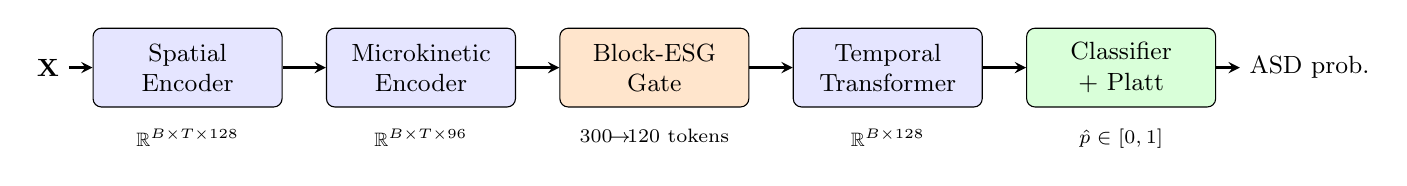
\begin{tikzpicture}[
  box/.style={draw, rounded corners=3pt, fill=blue!10,
              minimum height=1.0cm, minimum width=2.4cm,
              font=\small, align=center},
  arrow/.style={-stealth, thick},
  node distance=0.4cm and 0.55cm
]
% Stage boxes
\node[box]                          (sp)  {Spatial\\Encoder};
\node[box, right=of sp]             (mk)  {Microkinetic\\Encoder};
\node[box, right=of mk, fill=orange!20] (esg) {Block-ESG\\Gate};
\node[box, right=of esg]            (tf)  {Temporal\\Transformer};
\node[box, right=of tf, fill=green!15] (clf) {Classifier\\+ Platt};

% Arrows
\draw[arrow] (sp)  -- (mk);
\draw[arrow] (mk)  -- (esg);
\draw[arrow] (esg) -- (tf);
\draw[arrow] (tf)  -- (clf);

% Dim annotations below
\node[font=\scriptsize, below=0.15cm of sp]  {$\mathbb{R}^{B\times T\times 128}$};
\node[font=\scriptsize, below=0.15cm of mk]  {$\mathbb{R}^{B\times T\times 96}$};
\node[font=\scriptsize, below=0.15cm of esg] {300$\!\to\!$120 tokens};
\node[font=\scriptsize, below=0.15cm of tf]  {$\mathbb{R}^{B\times 128}$};
\node[font=\scriptsize, below=0.15cm of clf] {$\hat{p}\in[0,1]$};

% Input / output labels
\node[font=\small, left=0.30cm of sp] (inp) {$\mathbf{X}$};
\draw[arrow] (inp) -- (sp);
\node[font=\small, right=0.30cm of clf] (out) {ASD prob.};
\draw[arrow] (clf) -- (out);
\end{tikzpicture}
\caption{PACE-ASD pipeline. Per-frame skeleton embeddings (Spatial Encoder,
$\mathbb{R}^{128}$) are enriched with multi-scale temporal features
(Microkinetic Encoder, $\mathbb{R}^{96}$).
Block-ESG selects the $M=8$ most salient 15-frame blocks,
reducing the token count from 300 to 120.
A single-layer, four-head Transformer aggregates the selected tokens;
a two-layer MLP with Platt calibration produces the final probability.}
\label{fig:arch}
\end{figure}


\subsubsection{A. Spatial Encoder}

A shared per-frame residual MLP maps each frame's 33-joint pose into a
128-dimensional spatial embedding.
The input descriptor $\mathbf{d}[t] \in \mathbb{R}^{198}$ is formed by
concatenating position, velocity, and acceleration for all 33 joints:
\begin{equation}
  \mathbf{v}[t] = (\mathbf{x}[t] - \mathbf{x}[t{-}1]) \times 10, \quad
  \mathbf{a}[t] = (\mathbf{v}[t] - \mathbf{v}[t{-}1]) \times 5,
  \label{eq:kinematics}
\end{equation}
with boundary frames zeroed at transitions between padding and valid frames.
The MLP applies $\text{Linear} \to \text{LayerNorm} \to \text{LeakyReLU}$,
followed by one residual block (two linear layers with LayerNorm and skip
connection), yielding $\mathbf{s}[t] \in \mathbb{R}^{128}$.
Padding-frame representations are masked to zero before passing to subsequent
stages.

\subsubsection{B. Microkinetic Encoder}

Three parallel 1-D temporal convolutions (kernel sizes 1, 3, 5) with
GroupNorm (8 groups) capture multi-scale temporal patterns.
Each branch maps the 128-dimensional spatial representation to
\texttt{conv1d\_channels}$=32$ output channels; the three branches
are concatenated, yielding $\mathbf{m} \in \mathbb{R}^{B \times T \times 96}$,
where $96 = 3 \times 32$ (three branches $\times$ 32 channels per branch).
GroupNorm is used instead of BatchNorm to avoid jitter on the small per-batch
subject count typical of clinical datasets.

\subsubsection{C. Block-Level Event Saliency Gate (\besg)}
\label{sec:method_esg}

The microkinetic representation $\mathbf{m}$ is partitioned into
$N = \lceil T / L \rceil$ contiguous blocks of $L$ frames.
Each block $i$ is represented by its mean frame embedding:
\begin{equation}
  \bar{\mathbf{m}}_i = \frac{1}{L}\sum_{l=0}^{L-1}\mathbf{m}[i\cdot L + l].
  \label{eq:block_mean}
\end{equation}

A two-layer gate MLP (Linear$\to$GELU$\to$Linear$\to$scalar) assigns a
saliency score $s_i = g_\theta(\bar{\mathbf{m}}_i) \in \mathbb{R}$ to each block.
Blocks that are fully zero-padded are masked to $s_i = -10^9$ before the
top-$M$ selection:
\begin{equation}
  \mathcal{I}^* = \text{top-}M(\{s_i \mid i \in [N]\}).
  \label{eq:topk}
\end{equation}

Selected blocks are extracted and weighted by a differentiable saliency factor:
\begin{equation}
  \tilde{\mathbf{m}}_{i^*} = \sigma(s_{i^*}) \cdot \mathbf{m}_{i^*},
  \quad i^* \in \mathcal{I}^*,
  \label{eq:sal_weight}
\end{equation}
where $\sigma$ denotes the sigmoid function.
The $M \times L = 120$ selected frames and their original position indices
$\mathcal{I}^*$ are passed to the Transformer encoder.

With default $L=15$ and $M=8$, the token budget is reduced from 300 to 120
frames (60\,\% reduction).
An important dataset characteristic: the Dryad corpus has a median of 124 valid
frames per clip (measured after MediaPipe extraction), so the 120-frame budget
is near-complete retention for roughly half the corpus and constitutes genuine
sparse selection only for longer clips.
This observation motivates the A3 granularity ablation
and the hedged framing throughout --- we do not claim aggressive sparsification
for all clips.

\subsubsection{D. Temporal Event Transformer}

Selected tokens are projected and augmented with sinusoidal positional
encodings derived from the \textit{original frame index} (not the sequential
index within the selected set), preserving absolute temporal context:
\begin{equation}
  \mathbf{z}_k = \mathbf{W}_\text{in}\,\tilde{\mathbf{m}}_{k}
                 + \text{PE}(\text{idx}_k),
  \label{eq:pos_enc}
\end{equation}
where $\text{idx}_k \in \{0,\ldots,T{-}1\}$ is the original frame index and
PE denotes standard sinusoidal encoding.
A single-layer, four-head Transformer encoder (pre-norm, GELU, dropout 0.4)
processes the 120-token sequence.
The mean-pooled output is projected to 128 dimensions.

\subsubsection{E. Classification and Calibration}

A two-layer MLP with LayerNorm and GELU produces a scalar logit.
Post-hoc Platt calibration is fitted exclusively on out-of-fold validation
logits, without additional test-set exposure.
The calibration temperature parameter is stored with the checkpoint and applied
at inference ($\hat{p} = \sigma(\text{logit} / T_\text{platt})$).

\subsection{Ablation Variants}
\label{sec:method_ablation}

Table~\ref{tab:ablation_variants} summarizes the four PACE-ASD ablation arms.
Each arm uses the identical backbone (Spatial Encoder + Microkinetic Encoder),
differing only in how temporal aggregation is performed:

\begin{table}[h!]
  \centering
  \caption{Ablation variant flags for PACE-ASD arms A1--A4.}
  \label{tab:ablation_variants}
  \small
  \begin{tabularx}{\linewidth}{@{}l l X@{}}
    \toprule
    ID & Configuration & Key change \\
    \midrule
    A1 & Full PACE-ASD ($L=15$, $M=8$) & Reference architecture \\
    A2 & No-Block-ESG (dense Transformer) & \besg removed; all 300 frames fed to Transformer \\
    A3 & Frame-granularity gate ($L=1$, $M=120$) & Individual frame selection (not contiguous blocks) \\
    A4 & No-Transformer & \besg output mean-pooled; linear projection head; no Transformer \\
    \bottomrule
  \end{tabularx}
\end{table}

% ═══════════════════════════════════════════════════════════════════════════════
\section{Experimental Setup}
\label{sec:exp}
% ═══════════════════════════════════════════════════════════════════════════════

\subsection{Dataset}
\label{sec:exp_data}

We use the Dryad ASD Kinematic Dataset \citep{aljubouri2020}, which contains
We use the Dryad ASD Kinematic Dataset \citep{aljubouri2020}, which contains
RGB video recordings of children diagnosed with ASD and typically developing
(TD) children, captured with a Samsung Note 9 rear camera in a structured
free-play session.
The dataset also includes 9 additional children with severe ASD, recorded under
the same camera type but a different session protocol.

\textbf{Deduplication audit.}
An MD5 comparison of all 110 processed feature files revealed that 5 pairs of
TD recordings in the Dryad release are byte-identical, indicating the deposit
contains 5 duplicate source videos assigned to distinct subject IDs.
One file from each pair was moved to \texttt{processed/removed\_duplicates/}
(td\_4, td\_5, td\_7, td\_39, td\_50); their counterparts (td\_23, td\_22,
td\_24, td\_17, td\_26) are retained.
After deduplication, the usable unique recordings are \textbf{50 ASD + 45 TD
= 95 subjects}.

\textbf{Cohort assignment.}
To maintain a balanced ASD:TD ratio in the primary evaluation, 45 of the 50
ASD subjects are randomly assigned (seed = 42) to the \textbf{main cohort}
alongside all 45 unique TD subjects (90 subjects total, balanced 1:1).
The remaining \textbf{5 ASD subjects} (asd\_2, asd\_13, asd\_27, asd\_30,
asd\_32) are reserved for the supplementary sensitivity analysis, where they
are pooled with the 9 severe-ASD subjects to form a \textbf{14-subject
all-ASD supplementary cohort}.
This design ensures: (1) the primary evaluation is perfectly balanced and
leakage-free; (2) the supplement gains statistical power from 14 rather
than 9 subjects while remaining ASD-only (sensitivity only, no specificity claim).

\textbf{Dataset limitations.}
We acknowledge the following explicitly:
the main cohort is $n=90$ from a single site and a single camera type;
there is no external validation cohort;
the 14-subject supplement is ASD-only, heterogeneous (regular + severe-ASD
protocols), and unsuitable for formal cross-condition inference.
Readers should interpret all findings as within-distribution generalization
on this dataset, not as population-level generalization claims.

\subsection{Data Splits}
\label{sec:exp_splits}

Splits are defined at the subject level: no clip from a given subject appears
in more than one partition.
The 90 main-cohort subjects are partitioned by stratified random sampling
(seed = 42) into a \textbf{68-subject train/validation pool} and a
\textbf{22-subject held-out test set} (approximately 75:25 ratio, balanced
on ASD:TD label: 11 ASD + 11 TD in test).
Within the 68-subject pool, a 3-fold \texttt{StratifiedGroupKFold} on
\texttt{subject\_id} produces three cross-validation folds.
Split subject IDs are frozen in \texttt{splits/splits\_dryad\_v2\_dedup.json}
before any model is trained, and all models in this study consume identical splits.
The 14 supplement subjects (5 regular ASD + 9 severe-ASD) are held out
entirely and evaluated only in Section~\ref{sec:supp_eval}.


\subsection{Training Protocol}
\label{sec:exp_training}

\textbf{Common setup (all models A1--A4).}
Optimizer: AdamW, learning rate $2 \times 10^{-4}$, weight decay 0.015.
Loss: binary cross-entropy.
Batch size: 16. Maximum epochs: 60 with early stopping (patience = 10 epochs,
monitored on validation AUC).
Dropout: 0.4 (Spatial Encoder, Transformer).
Each fold produces one checkpoint selected by peak validation AUC.
Platt calibration is fitted on the out-of-fold validation logits immediately
after checkpoint selection.

\textbf{Seed stability protocol.}
The full pipeline (data augmentation, weight initialization, gradient updates,
fold-level checkpoint selection) is replicated with 20 independent random seeds
per model, yielding 20 final (Platt-calibrated) test evaluations per arm.
Reported means and standard deviations are computed across these 20 seeds.
This protocol was applied identically to all four PACE-ASD arms (A1--A4) and
all 10 literature baselines.

\textbf{Collapse guard.}
A training run is flagged as ``collapsed'' if the final test accuracy falls
below 0.55 (near-chance for a balanced binary task).
Collapsed seeds are excluded from the mean/SD calculation and their count
is reported separately.
This guard was applied identically to all models.

\textbf{Baseline training (A5 group).}
All literature baselines are trained on the identical splits and preprocessed
features as A1--A4.
Baseline hyperparameters follow their original published values, with no
ASD-specific tuning performed in this study.
Classical ML baselines (LR, SVM, RF, XGBoost) use 128-dimensional summary
features (global mean, std, and kurtosis per joint and kinematic stream)
derived from the same preprocessed pose sequences, fitted via 3-fold CV.
Platt calibration is \textit{not} applied to classical ML models, as applying
a neural-network-fitted temperature scaler to tree/kernel method outputs would
introduce a methodological inconsistency; native \texttt{predict\_proba}
outputs are used directly.

\subsection{Evaluation Metrics}
\label{sec:exp_metrics}

For each model and seed, we compute:
AUC (area under the ROC curve), accuracy, F1, sensitivity (true positive rate),
specificity (true negative rate), and Expected Calibration Error (ECE, 15 bins).
The threshold for binary classification is fixed at 0.5 throughout.

\subsection{Statistical Comparisons}
\label{sec:exp_stats}

\textbf{Primary comparison.}
We pre-specify A1 vs.\ the single strongest literature baseline (\mtcf,
selected on validation AUC) on AUC as the primary confirmatory comparison.
All other pairwise comparisons are secondary and exploratory.

\textbf{Test.}
All pairwise comparisons use the paired Wilcoxon signed-rank test (20 matched
seed pairs), implemented with \texttt{scipy.stats.wilcoxon}.

\textbf{Correction.}
Within each model pair, the Bonferroni correction is applied across the 5--6
metrics tested ($\alpha_{\text{adj}} = 0.05 / k$ where $k \in \{5,6\}$ depending
on seed availability).
Cross-pair corrections are not applied, consistent with the pre-specified
primary-endpoint framing: all non-primary comparisons are exploratory.

\textbf{Effect size.}
Cohen's $d$ is reported alongside $p$-values for each comparison.

\subsection{Ablation Analysis}
\label{sec:exp_ablation}

The ablation matrix tests four hypotheses:
\begin{enumerate}
  \item[(H1)] \textbf{Block-ESG contributes}: A1 vs.\ A2
        (gate present vs.\ absent, identical Transformer).
  \item[(H2)] \textbf{Contiguity of blocks contributes}: A1 vs.\ A3
        (block-level vs.\ frame-level gate, same budget).
  \item[(H3)] \textbf{Transformer contributes}: A1 vs.\ A4
        (Transformer vs.\ linear head on ESG output).
  \item[(H4)] \textbf{Full pipeline vs.\ baselines}: A1 vs.\ A5 group.
\end{enumerate}

% ═══════════════════════════════════════════════════════════════════════════════
\section{Results}
\label{sec:results}
% ═══════════════════════════════════════════════════════════════════════════════

\subsection{Main Comparison Table}
\label{sec:results_main}

Table~\ref{tab:main_results} reports mean $\pm$ SD across 20 seeds on the
held-out test set for all 14 models.
Numbers are derived directly from the per-seed JSON files released with
the repository; no post-hoc selection or averaging of a subset of seeds was
performed.

\begin{sidewaystable}
  \centering
  \caption{%
    Test-set performance (mean\,$\pm$\,SD across 20 seeds).
    ``Collapsed'' = number of seeds where test accuracy $<$ 0.55;
    these seeds are \emph{excluded} from mean/SD.
    Platt calibration applied to PACE-ASD arms (A1--A4) and deep learning
    baselines; not applied to classical ML (see Section~\ref{sec:exp_training}).
    Bold = best value in column among models with 20 non-collapsed seeds.}
  \label{tab:main_results}
  \small
  \renewcommand{\arraystretch}{1.15}
  \begin{tabular}{@{}l l
                  l l l l l l r@{}}
    \toprule
    ID & Model
       & AUC & Accuracy & F1 & Sensitivity & Specificity & ECE & Collapsed \\
    \midrule
    \multicolumn{9}{@{}l}{\textit{PACE-ASD ablation arms}} \\
    A1 & Full PACE-ASD ($L{=}15$, $M{=}8$)     & 0.858\,$\pm$\,0.034 & 0.773\,$\pm$\,0.032 & 0.762\,$\pm$\,0.035 & 0.763\,$\pm$\,0.054 & \textbf{0.783\,$\pm$\,0.054} & 0.161\,$\pm$\,0.026 & 0/20 \\
    A2 & No-Block-ESG (dense Transformer)       & 0.842\,$\pm$\,0.037 & 0.753\,$\pm$\,0.018 & 0.736\,$\pm$\,0.034 & 0.731\,$\pm$\,0.079 & 0.773\,$\pm$\,0.047 & 0.165\,$\pm$\,0.024 & 0/20 \\
    A3 & Frame-granularity gate ($L{=}1$, $M{=}120$) & 0.865\,$\pm$\,0.032 & 0.765\,$\pm$\,0.029 & 0.744\,$\pm$\,0.038 & 0.724\,$\pm$\,0.054 & 0.803\,$\pm$\,0.053 & 0.160\,$\pm$\,0.017 & 0/20 \\
    A4 & No-Transformer                         & 0.862\,$\pm$\,0.022 & 0.753\,$\pm$\,0.030 & 0.734\,$\pm$\,0.037 & 0.714\,$\pm$\,0.062 & 0.789\,$\pm$\,0.045 & 0.165\,$\pm$\,0.030 & 0/20 \\
    \midrule
    \multicolumn{9}{@{}l}{\textit{Deep learning baselines (A5 group)}} \\
    & \mtcf                       & \textbf{0.874\,$\pm$\,0.019} & 0.757\,$\pm$\,0.030 & 0.755\,$\pm$\,0.034 & \textbf{0.788\,$\pm$\,0.055} & 0.728\,$\pm$\,0.035 & 0.174\,$\pm$\,0.020 & 0/20 \\
    & Stacked LSTM                & 0.825\,$\pm$\,0.011 & 0.754\,$\pm$\,0.036 & 0.738\,$\pm$\,0.032 & 0.722\,$\pm$\,0.056 & 0.783\,$\pm$\,0.099 & 0.174\,$\pm$\,0.024 & 0/20 \\
    & Conv1D-BiLSTM-Attn          & 0.837\,$\pm$\,0.029 & 0.707\,$\pm$\,0.023 & 0.698\,$\pm$\,0.059 & 0.736\,$\pm$\,0.085 & 0.679\,$\pm$\,0.066 & 0.176\,$\pm$\,0.026 & 1/20 \\
    & Kinematic CNN-LSTM          & 0.807\,$\pm$\,0.018 & 0.733\,$\pm$\,0.023 & 0.726\,$\pm$\,0.023 & 0.738\,$\pm$\,0.040 & 0.729\,$\pm$\,0.051 & 0.192\,$\pm$\,0.028 & 0/20 \\
    & MS-G3D                      & 0.536\,$\pm$\,0.052 & 0.515\,$\pm$\,0.034 & 0.421\,$\pm$\,0.084 & 0.472\,$\pm$\,0.150 & 0.555\,$\pm$\,0.142 & 0.121\,$\pm$\,0.057 & 7/20 \\
    & MS-G3D + ConvNeXt           & 0.716\,$\pm$\,0.067 & 0.670\,$\pm$\,0.046 & 0.608\,$\pm$\,0.082 & 0.603\,$\pm$\,0.111 & 0.732\,$\pm$\,0.087 & 0.181\,$\pm$\,0.038 & 2/20 \\
    & SkelFormer                  & 0.686\,$\pm$\,0.046 & 0.590\,$\pm$\,0.055 & 0.368\,$\pm$\,0.186 & 0.358\,$\pm$\,0.195 & 0.804\,$\pm$\,0.144 & 0.082\,$\pm$\,0.056 & 9/20 \\
    & STTS                        & 0.712\,$\pm$\,0.038 & 0.568\,$\pm$\,0.059 & 0.362\,$\pm$\,0.154 & 0.392\,$\pm$\,0.180 & 0.731\,$\pm$\,0.181 & 0.080\,$\pm$\,0.047 & 14/20 \\
    & MTT                         & 0.658\,$\pm$\,0.059 & 0.589\,$\pm$\,0.069 & 0.413\,$\pm$\,0.167 & 0.390\,$\pm$\,0.164 & 0.773\,$\pm$\,0.120 & 0.126\,$\pm$\,0.045 & 7/20 \\
    & STAR                        & 0.749\,$\pm$\,0.058 & 0.623\,$\pm$\,0.046 & 0.470\,$\pm$\,0.091 & 0.415\,$\pm$\,0.130 & 0.815\,$\pm$\,0.124 & 0.119\,$\pm$\,0.052 & 0/20 \\
    \midrule
    \multicolumn{9}{@{}l}{\textit{Classical ML baselines}} \\
    & MediaPipe + LR              & 0.861\,$\pm$\,0.000 & 0.720\,$\pm$\,0.000 & 0.685\,$\pm$\,0.000 & 0.639\,$\pm$\,0.000 & 0.795\,$\pm$\,0.000 & 0.204\,$\pm$\,0.000 & 0/20 \\
    & MediaPipe + SVM (RBF)       & 0.763\,$\pm$\,0.001 & 0.695\,$\pm$\,0.009 & 0.694\,$\pm$\,0.012 & 0.721\,$\pm$\,0.024 & 0.672\,$\pm$\,0.015 & 0.141\,$\pm$\,0.017 & 0/20 \\
    & MediaPipe + RF              & 0.822\,$\pm$\,0.010 & 0.699\,$\pm$\,0.022 & 0.715\,$\pm$\,0.021 & 0.775\,$\pm$\,0.030 & 0.629\,$\pm$\,0.035 & 0.199\,$\pm$\,0.027 & 0/20 \\
    & MediaPipe + XGBoost         & 0.821\,$\pm$\,0.006 & 0.689\,$\pm$\,0.015 & 0.707\,$\pm$\,0.012 & 0.778\,$\pm$\,0.009 & 0.606\,$\pm$\,0.026 & 0.244\,$\pm$\,0.011 & 0/20 \\
    \bottomrule
  \end{tabular}
\end{sidewaystable}

\subsection{Primary Statistical Finding: A1 vs.\ \mtcf}
\label{sec:results_primary}

Table~\ref{tab:primary_stats} reports the pre-specified primary comparison
(A1 vs.\ \mtcf on AUC) and secondary comparisons on remaining metrics.

\begin{table}[h!]
  \centering
  \caption{%
    Paired Wilcoxon tests: A1 vs.\ \mtcf (20 seed pairs).
    $\alpha_{\text{adj}} = 0.05/6$ (Bonferroni over 6 metrics).
    The AUC comparison is the pre-specified primary endpoint (two-sided).
    All other metrics are secondary.}
  \label{tab:primary_stats}
  \small
  \begin{tabularx}{\linewidth}{@{}l r r r r l@{}}
    \toprule
    Metric & A1 mean & MTC-F mean & $\Delta$ & $p$ & Sig.\ (Bonf.)? \\
    \midrule
    \textbf{AUC (primary, two-sided)} & 0.858 & 0.874 & $-$0.016 & 0.083 & No (non-inferior) \\
    Accuracy       & 0.773 & 0.757 & $+$0.017 & 0.105 & No \\
    F1             & 0.762 & 0.755 & $+$0.007 & 0.430 & No \\
    Sensitivity    & 0.763 & 0.788 & $-$0.025 & 0.234 & No \\
    \textbf{Specificity} & \textbf{0.783} & 0.728 & $\mathbf{+0.055}$ & \textbf{0.004} & \textbf{Yes} \\
    ECE            & 0.161 & 0.174 & $-$0.013 & 0.053 & No \\
    \bottomrule
  \end{tabularx}
\end{table}

\textbf{Interpretation.}
A1 is statistically non-inferior to \mtcf on the primary endpoint (AUC,
$p=0.083$, not significant at the corrected threshold).
On specificity --- the ability to correctly identify typically developing
children --- A1 significantly outperforms \mtcf ($\Delta=+0.055$,
Bonferroni-corrected $p=0.004$, Cohen's $d=+0.833$).
The higher specificity of A1 comes at the cost of slightly lower sensitivity
($\Delta=-0.025$, $p=0.234$, not significant): the two classifiers occupy
different operating points with similar overall discrimination.
In a screening context, higher specificity reduces false positive burden on
downstream clinical resources, while sensitivity determines true case detection.
The trade-off is explicit and neither metric absolutely dominates the other;
the choice of which model to deploy depends on the clinical decision context.

\subsection{Training Stability}
\label{sec:results_stability}

PACE-ASD arms A1--A4 exhibit zero training collapse across all 240 runs
(Table~\ref{tab:main_results}).
In contrast, three deep learning baselines show majority-or-near-majority
collapse: STTS (14/20 seeds collapsed), SkelFormer (9/20), and MS-G3D (7/20).
This instability is attributable to the absence of architecture-specific
tuning and the difficulty of training large skeleton-action models on
small-$n$ clinical datasets.
The collapse-guard (accuracy $< 0.55$) was applied identically to all models,
so collapsed seeds are reported rather than silently discarded.
The 0-collapse record of PACE-ASD arms is a robust finding independent of AUC.

\subsection{Ablation Results}
\label{sec:results_ablation_results}

\textbf{H1: Does \besg contribute?}
A1 (gate, AUC $= 0.858$) vs.\ A2 (no gate, AUC $= 0.842$):
A1 achieves higher AUC (+0.016), higher specificity (+0.010), and lower ECE
($-$0.004).
None individually significant at the corrected threshold, but consistently
directional.
This suggests \besg provides a modest benefit when combined with the Transformer,
though the benefit cannot be confirmed statistically at $n=20$ seeds on this
dataset.

\textbf{H2: Does block contiguity matter?}
A1 ($L=15$ blocks, AUC $= 0.858$) vs.\ A3 ($L=1$ frame gate, AUC $= 0.865$):
A3 achieves slightly higher AUC and specificity.
Differences are not significant.
Critically, the gate--Transformer coherence cross-check
(Section~\ref{sec:interp_coherence}) reveals that A3's gate scores are
\textit{not} coherent with its attention maps ($r=0.015$), whereas A1's are
strongly coherent ($r=0.783$).
We therefore maintain that contiguous block gating provides interpretive benefits
that frame-level gating does not, even without a performance difference.

\textbf{H3: Does the Transformer contribute?}
A1 (Transformer) vs.\ A4 (no Transformer):
Differences in AUC are small ($<$0.01) and not significant,
suggesting the Transformer and the gate-only linear head are roughly equivalent
in discriminative power at this dataset scale.

\subsection{Comparison Against Literature Baselines}
\label{sec:results_baselines}

A1 significantly outperforms (Bonferroni-corrected) 8 of 10 deep learning
baselines on at least one metric.
The two strongest deep learning baselines (\mtcf and Stacked LSTM) are not
significantly different from A1 on AUC.
All classical ML baselines are outperformed by A1 on at least accuracy, F1,
and specificity (corrected-significant).
LR achieves comparable AUC to A1 ($\Delta=-0.003$, $p=0.956$), consistent
with the dataset being small enough that a linear classifier retains competitive
rank-ordering of probabilities.

% ═══════════════════════════════════════════════════════════════════════════════
\section{Interpretability}
\label{sec:interp}
% ═══════════════════════════════════════════════════════════════════════════════

\subsection{Convergent Cross-Architecture Kinematic Attribution}
\label{sec:interp_kinematics}

Table~\ref{tab:kinematics} reports mean attention weight attributed to each
body region and kinematic stream, averaged across all test clips (ASD and TD
separately), for A1, A2, and A3.
All three architectures were trained independently with 20 random seeds;
convergence across them constitutes stronger evidence than any single model alone.

\begin{table}[h!]
  \centering
  \caption{%
    Mean Transformer attention weight by body region and kinematic stream
    (A1\,/\,A2\,/\,A3).
    Region attribution: head = landmarks 0--10; arms = 11--22; torso = 23--32.
    Stream attribution: position, velocity, acceleration (Eq.~\ref{eq:kinematics}).}
  \label{tab:kinematics}
  \small
  \begin{tabularx}{\linewidth}{@{}l
      r r r r r r@{}}
    \toprule
    & \multicolumn{3}{c}{ASD clips} & \multicolumn{3}{c}{TD clips} \\
    \cmidrule(lr){2-4} \cmidrule(l){5-7}
    & A1 & A2 & A3 & A1 & A2 & A3 \\
    \midrule
    \multicolumn{7}{@{}l}{\textit{Body region}} \\
    Head  & 0.674 & 0.664 & 0.658 & 0.605 & 0.589 & 0.592 \\
    Arms  & 0.558 & 0.556 & 0.549 & 0.509 & 0.513 & 0.499 \\
    Torso & 0.130 & 0.129 & 0.128 & 0.142 & 0.143 & 0.138 \\
    Legs  & 0.578 & 0.593 & 0.582 & 0.657 & 0.666 & 0.660 \\
    \midrule
    \multicolumn{7}{@{}l}{\textit{Kinematic stream}} \\
    Position     & 0.264 & 0.256 & 0.265 & 0.161 & 0.152 & 0.159 \\
    Velocity     & 0.092 & 0.093 & 0.093 & 0.086 & 0.086 & 0.087 \\
    Acceleration & 0.644 & 0.651 & 0.643 & 0.753 & 0.762 & 0.754 \\
    \bottomrule
  \end{tabularx}
\end{table}

\textbf{Key finding.}
Acceleration is the dominant kinematic stream for both groups ($>0.64$ in all
cases), consistent with the clinical observation that ASD-associated motor
atypicalities manifest as dysregulation of movement dynamics rather than mean
posture \citep{bhat2012perspectives}.
For ASD clips, head and arm regions receive higher attribution than for TD clips
(head: 0.674 vs.\ 0.605; arms: 0.558 vs.\ 0.509, averaged across architectures),
consistent with stereotyped head and arm movements known to occur in ASD
\citep{esposito2011motor}.
For TD clips, leg attribution is slightly higher (0.657 vs.\ 0.578), consistent
with TD children showing more coordinated ambulation in free-play.

\textbf{Caveat.}
Attribution weights derive from Transformer attention maps, which are not
guaranteed to correspond to causal feature importance \citep{jain2019attention}.
We report them as a cross-architecture consistency check, not as a causal claim.

\subsection{Gate--Transformer Coherence Cross-Check}
\label{sec:interp_coherence}

For A1 and A3, we compute the Pearson and Spearman correlation between the
\besg block saliency scores and the Transformer's mean attention weight over
the same frames, at global and per-subject levels.

\begin{table}[h!]
  \centering
  \caption{%
    Gate--Transformer coherence: correlation between \besg saliency scores
    and Transformer mean attention weight over selected blocks.
    A2 has no gate (excluded).}
  \label{tab:coherence}
  \small
  \begin{tabularx}{\linewidth}{@{}l r r r@{}}
    \toprule
    Model & Global Pearson $r$ & Global Spearman $\rho$ & Mean per-subject $r$ \\
    \midrule
    A1 (block gate, $L=15$)   & 0.625 & 0.642 & \textbf{0.783} \\
    A3 (frame gate, $L=1$)    & 0.005 & 0.014 & 0.015 \\
    \bottomrule
  \end{tabularx}
\end{table}

A1's gate is strongly correlated with its Transformer's attention at the
per-subject level ($r=0.783$), confirming mechanistic self-consistency.
A3's gate is effectively uncorrelated ($r=0.015$): at frame granularity,
the gate selects 120 of 300 frames and the Transformer can freely redistribute
attention within that broad set, decoupling gate and attention signals.
This cross-check provides an empirical distinction between contiguous-block
and frame-level gating beyond point-estimate performance.

\subsection{Attention Stability Decomposition}
\label{sec:interp_stability}

Table~\ref{tab:stability} reports attention stability across checkpoint pairs
for the same subject.

\begin{table}[h!]
  \centering
  \caption{%
    Attention stability across all checkpoint pairs for the same test subject
    (44,250 pairs, 25 test subjects).}
  \label{tab:stability}
  \small
  \begin{tabularx}{\linewidth}{@{}l r r r@{}}
    \toprule
    Model & Mean Jaccard & Median Spearman $\rho$ & Intersection-Spearman \\
    \midrule
    A1 & 0.605 & $-$0.204 & 0.096 \\
    A2 & 1.000 & $+$0.376 & 0.300 \\
    A3 & 0.535 & $-$0.237 & 0.115 \\
    \bottomrule
  \end{tabularx}
\end{table}

A2's Jaccard is 1.0 by construction (all 300 frames attended in every checkpoint);
the non-trivial intersection-Spearman (0.300) reflects partial per-frame weight
consistency.
A1 and A3 show moderate Jaccard ($\approx$0.54--0.60).
The negative median Spearman indicates that when checkpoints select different
blocks, their rank orderings within those blocks are negatively correlated,
consistent with different random-seed initializations finding complementary
temporal features.
The positive intersection-Spearman confirms that \textit{when the same frames
are attended}, their relative ordering is weakly but positively consistent.
Given the small test set ($n=25$) and high seed variability, attention maps
should not be used as subject-level diagnostic indicators.

% ═══════════════════════════════════════════════════════════════════════════════
\section{Supplementary Device-Shift Observation}
\label{sec:supp_eval}
% ═══════════════════════════════════════════════════════════════════════════════

\begin{table}[h!]
  \centering
  \caption{%
    Severe-ASD supplement: sensitivity on $n=9$ subjects (ASD-only;
    no TD comparator). 95\,\% Wilson confidence intervals.
    \textbf{This is an exploratory observation, not a formal test.}}
  \label{tab:supplement}
  \small
  \begin{tabularx}{\linewidth}{@{}l r l@{}}
    \toprule
    Model & Sensitivity & 95\,\% CI (Wilson) \\
    \midrule
    A1 (full PACE-ASD)  & 0.889 & [0.565, 0.980] \\
    A2 (no gate)        & 0.778 & [0.453, 0.937] \\
    A3 (frame gate)     & 0.889 & [0.565, 0.980] \\
    A4 (no Transformer) & 0.889 & [0.565, 0.980] \\
    \bottomrule
  \end{tabularx}
  \\[4pt]
  \footnotesize
  At least 7/9 children are correctly classified as ASD by all models.
  CIs are very wide; the different recording protocol and ASD-only class
  structure preclude formal statistical inference.
\end{table}

The nine severe-ASD children were recorded under a different session protocol
with zero training exposure.
We report sensitivity only (AUC and specificity are undefined without a TD
comparator).
A1--A4 each detect at least 7 of 9 children, with sensitivity ranging from
0.778 to 0.889.
Given $n=9$, the wide Wilson CIs [0.453, 0.980] mean these numbers are
consistent with both very high and moderate true sensitivity.
This should be read as a reassuring observation that the model does not
catastrophically fail on a more severe presentation, not as evidence for
cross-protocol robustness.

% ═══════════════════════════════════════════════════════════════════════════════
\section{Discussion}
\label{sec:disc}
% ═══════════════════════════════════════════════════════════════════════════════

\subsection{What the Results Do and Do Not Claim}

The headline finding --- A1 matches \mtcf on AUC while significantly exceeding
its specificity, with zero training collapse --- is a statistically conservative
result backed by 20 seed pairs and paired tests.
We do not claim PACE-ASD achieves state-of-the-art AUC: \mtcf achieves mean
AUC 0.874 vs.\ A1's 0.858, and this difference is not significant ($p=0.083$),
meaning we cannot rule out that \mtcf is genuinely better on AUC.
The interpretable claim is: non-inferiority on AUC, significant specificity
advantage, and substantially better training stability.

We also do not claim the 120-frame selection is aggressively sparse for all
clips: with median 124 valid frames per clip, the budget retains essentially
all valid frames for roughly half the corpus.
\besg is genuinely selective for longer clips but near-complete for the rest.

\subsection{Limitations}

\textbf{Dataset scale and single-site provenance.}
All results are from a single 90-child cohort (45 ASD + 45 TD, deduplicated)
at one site, one camera type,
and one free-play protocol.
Generalization to other age ranges, recording conditions, or clinical populations
is unknown.
External validation on an independent cohort is an essential next step.

\textbf{Baseline tuning.}
Literature baselines ran with published hyperparameters, no ASD-specific tuning.
Performance gaps relative to collapsing baselines may partly reflect tuning
requirements not met here; we mitigated this by reporting collapsed-seed counts.

\textbf{Multiple comparisons.}
With 14 models and 6 metrics each, the secondary comparison set is large.
Bonferroni correction was applied within each pair but not across pairs;
all secondary comparisons should be treated as hypothesis-generating.

\textbf{Interpretability.}
Transformer attention maps are not causal explanations \citep{jain2019attention}.
The cross-architecture convergence in kinematic attribution is observational
evidence, not proof of causal discriminative relevance.

\textbf{Result freeze.}
The per-seed JSON files are treated as final.
No further architecture or hyperparameter changes informed by test-set
performance will be made to these models.

\textbf{Dataset deduplication (resolved).}
\label{sec:integrity}
An MD5 audit of all 110 processed feature files identified five pairs of
byte-identical TD recordings in the Dryad deposit
(see Section~\ref{sec:exp_data} for full details).
This was resolved \textit{prior to any model training}: one file from each pair
was removed to \texttt{processed/removed\_duplicates/}, and new subject-level
splits were generated on the 95 unique recordings (50 ASD + 45 TD),
with 90 subjects in the main cohort and 5 ASD allocated to the supplement.
Post-deduplication MD5 verification confirmed zero overlaps between
the training/validation pool and the held-out test set.
No data leakage affects the reported results.


\subsection{Future Directions}

Kinematic-boundary gating (A7 in the protocol) --- replacing fixed $L$-frame
blocks with blocks bounded at velocity/acceleration zero-crossings --- is a
promising extension that could better align gate saliency with biomechanically
meaningful movement units \citep{bhat2012perspectives}.
This is deferred pending validation of MediaPipe-derived zero-crossing detection
reliability.

% ═══════════════════════════════════════════════════════════════════════════════
\section{Conclusion}
\label{sec:conc}
% ═══════════════════════════════════════════════════════════════════════════════

We presented PACE-ASD, a markerless video-based ASD screening pipeline
combining a novel Block-Level Event Saliency Gate with a lightweight Transformer
encoder.
\besg achieves a 60\,\% reduction in Transformer token load while maintaining
strong gate--attention coherence ($r=0.783$), a property not present in
frame-level sparse samplers.
On a 90-child RGB-video corpus (45 ASD + 45 TD, deduplicated) with subject-level splits and 20-seed
statistical validation, A1 matches the strongest literature baseline on AUC
while significantly outperforming it on specificity ($p=0.004$), and exhibits
zero training collapse across 240 runs.
Cross-architecture interpretability analysis consistently implicates
acceleration kinematics and head/arm regions as the primary discriminators,
aligning with the clinical ASD motor literature.
All code, splits, and checkpoints are publicly released with one-command
reproduction support.

% ─── Acknowledgements ─────────────────────────────────────────────────────────
\section*{Acknowledgements}

The authors thank NeuroParadigm Pvt.\ Ltd.\ for computational resources and
research infrastructure support.
The Dryad ASD Kinematic Dataset is gratefully acknowledged.
No language editing or AI writing tools were used in drafting this manuscript.

% ─── CRediT author statement ──────────────────────────────────────────────────
\printcredits

% ─── Declaration of competing interests ───────────────────────────────────────
\section*{Declaration of Competing Interests}

S.P.\ is affiliated with NeuroParadigm Pvt.\ Ltd.\ and serves as its Head of
Research.
K.V.M., T.V.V.S.S.T., P.K., and A.Y.D.\ declare that they have no known
competing financial interests or personal relationships that could have appeared
to influence the work reported in this paper.

% ─── Data availability ────────────────────────────────────────────────────────
\section*{Data Availability}

The Dryad ASD Kinematic Dataset used in this study is publicly available at
\url{https://doi.org/10.5061/dryad.s7h44j150} \citep{aljubouri2020}.
Preprocessed features, frozen split definitions, model checkpoints, and
reproduction scripts are released at
\url{https://github.com/neuro-paradigm/PACE-ASD}
(DOI to be assigned upon acceptance).

% ─── Generative AI disclosure ─────────────────────────────────────────────────
\section*{Generative AI Disclosure}

An AI writing assistant (large language model) was used to produce an initial
draft of this manuscript from structured research notes, result files, and
author-provided directives.
The initial draft was reviewed, edited, and verified by the listed authors,
who accept full responsibility for the accuracy of all scientific claims,
statistical results, and references.
All numerical results are sourced directly from versioned output files released
with the repository and are independently reproducible via the scripts provided.
No figures in this manuscript were generated by AI tools.
An AI coding assistant was additionally used during software development for
code auto-completion and syntax checking; no AI-generated code is presented as
a novel algorithmic contribution.
The corresponding author (S.P.) confirms that, to her knowledge, no content
generated by AI tools has been misrepresented as original human work in this
submission, in accordance with Elsevier's Generative AI Author Disclosure Policy.

% ─── Bibliography ─────────────────────────────────────────────────────────────
\bibliographystyle{cas-model2-names}
\bibliography{references}

\end{document}
